\setlength{\footskip}{8mm}

\chapter{EXPERIMENT}

\begin{figure}[hbt!]
\caption{Experiments of source task knowledge learning}
\centerline{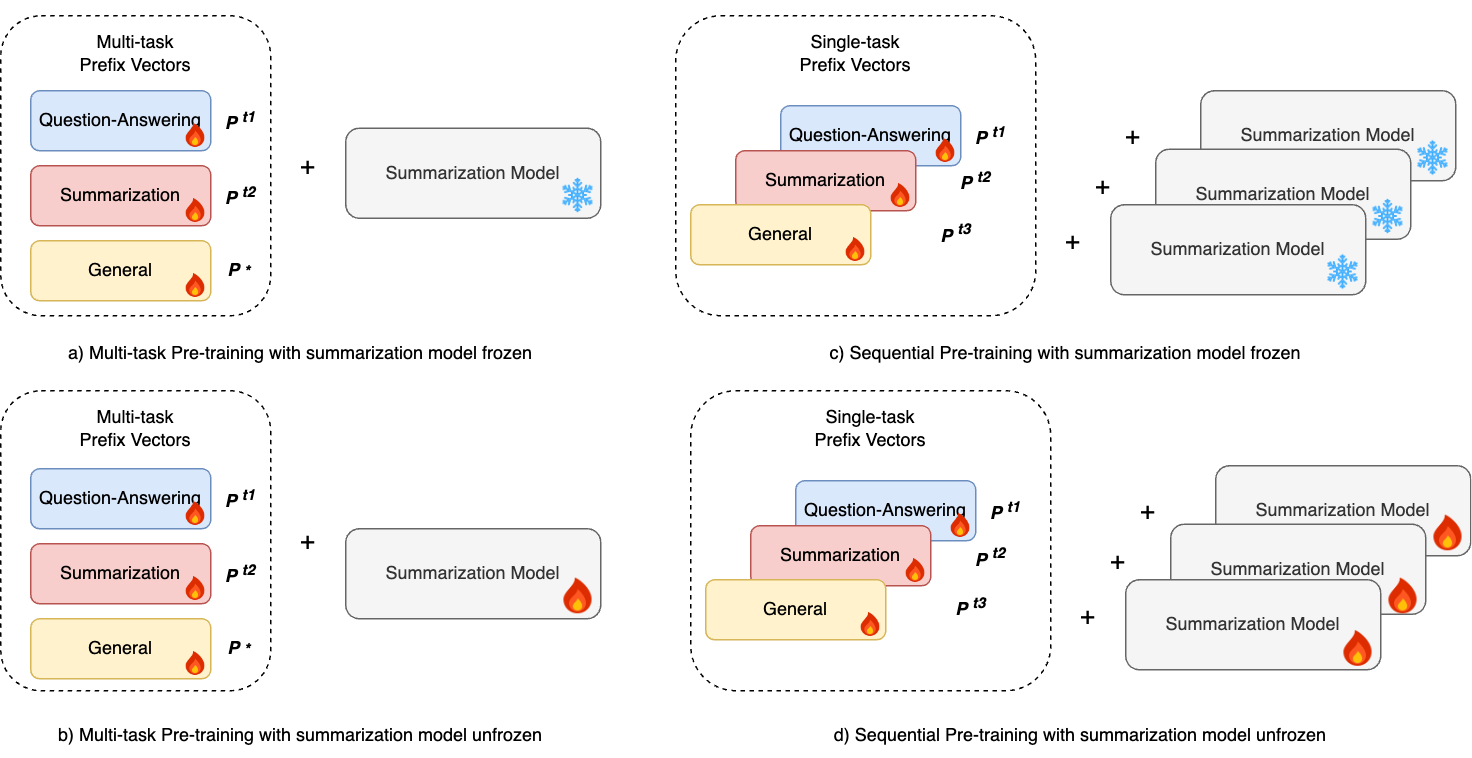
\includegraphics[width=15cm]{figures/phase1.png}}
\label{fig:phase1}
\small{\textit{Note.} Above displays comparison between experiments under multi-task vs single task and frozen vs unfrozen pre-trained model. Note that for each of the experiment, the presence vs absence of shared-task prefix. This will result in total of eight experiments. Additionally, an optimal number of prefix tokens are also experimented.}
\end{figure}

\textbf{If you are AI-related study,  this structure can be a good start.   You do NOT have to follow this, but completely swaying away from this structure must be with good reason:
}

\section{Rationale}
Explain again your key rationale and goals of your experiment.  This is to help readers understand your key idea that drives how you design your experiment.

\section{Dataset}
Explain the dataset you used.

\section{Experiment Setting}

\subsection{Preprocessing}
Explain the preprocessing techniques.

\subsection{Models/Techniques}
Explain the models/techniques you propose, or will compare or used in your work.

Write equations (way to reference - Eq \ref{eq:1}):

\begin{equation}
L(\theta , \theta_{p}) = \sum_{i}^{|Y|} log \mathbb{P}(y_{i} | X, y_{1}, ..., y_{i-1}) 
\label{eq:1}
\end{equation}

\subsection{Training}
Explain the training procedure in details so other can reproduce.

\subsection{Evaluation Metrics}
Explain clealry your evaluation metrics

\section{Other things}
Any other thing Chaky forgets or is only related to your work


\setcounter{section}{0}
\textbf{If you are user-study or HCI study,  follow this structure:
}

\section{Rationale}
Explain again your key rationale and goals of your experiment.  This is to help readers understand your key idea that drives how you design your methodology.

\section{Participants}
How many?  female, male,  demographics, right-handed-left-handed, etc.   Anything demographic that may influence your work should be stated here.

\section{Apparatus}
What instruments are used here?  Questionnaires?  Eye-tracking? Etc.

\section{Experimental Design}
IV, blocks, trials, duration, etc.

\section{Task and Procedure}
What are the tasks?  Procedure starting from inviting the participants to the lab,  they sign the consent, etc.

\section{Evaluation Metrics}
How you evaluate your work,  basically your DVs.

\section{Others}
Anything Chaky forgets or things only related to your work.
